\documentclass[UTF8]{ctexart}
\usepackage{mathtools,wallpaper}
\usepackage{hyperref} % For hyperlinks
\usepackage{t1enc}
\usepackage{pagecolor}
\usepackage{graphicx}
\usepackage{float}
\usepackage[margin=1in]{geometry} % 设置页边距

\begin{document}
\sloppy
	
\title{2024程序设计实训大作业项目文档}
\author{ 
    姓名:顾一马 \\ % 替换为你的姓名
    学号: 2023012827 \\ % 学号
    \href{mailto:gu-ym23@mails.tsinghua.edu.cn}{邮箱:gu-ym23@mails.tsinghua.edu.cn} % 邮箱地址
}
\date{2024-09-05}

\maketitle

\tableofcontents
\newpage

\section{模块之间的逻辑关系}
该游戏项目由多个模块组成,每个模块负责不同的功能。以下是主要模块及其关系的概述:

\begin{itemize}
    \item \textbf{主模块} (\texttt{MyGame.cpp, MyGame.h}): 负责游戏的主窗口和整体控制。它初始化游戏场景并管理游戏的主要流程。
    \item \textbf{场景模块} (\texttt{Scene.cpp, BattleScene.cpp}): 负责定义不同的游戏场景,例如战斗场景。场景模块管理游戏循环、时间管理、输入处理、对象移动和拾取操作,并通过 \texttt{update()} 方法进行定期更新。
    \item \textbf{角色模块} (\texttt{Character.cpp, Character.h, Link.cpp, Link.h}): 定义游戏中的角色,如主角和敌人。角色模块处理角色的状态、动作和交互,包括移动、拾取物品和管理装备。
    \item \textbf{装备模块} (\texttt{Armor.cpp, Armor.h, OldShirt.cpp, OldShirt.h}): 处理角色装备和道具的逻辑,包括防具和武器。装备模块还涉及到角色的防御和其他状态效果。
    \item \textbf{武器模块} (\texttt{Weapon.cpp, Weapon.h, Sword.cpp, Sword.h}): 定义不同类型的武器及其行为,例如剑和弓。每种武器都有独特的攻击方式和效果。
    \item \textbf{作弊码模块} (\texttt{CheatCodeManager.cpp, CheatCodeManager.h, CheatCodeDialog.cpp, CheatCodeDialog.h}): 提供作弊码的管理和输入界面功能,允许玩家在游戏中使用特殊功能。
    \item \textbf{地图模块} (\texttt{Map.cpp, Map.h, Battlefield.cpp, Battlefield.h}): 负责游戏中地图的创建和管理,包括地图布局、障碍物和地形特征。
    \item \textbf{平台模块} (\texttt{Platform.cpp, Platform.h}): 定义游戏中的不同类型的平台及其特性,例如木平台和金属平台。平台模块管理场景中的所有可踩踏物体。
    \item \textbf{特效模块} (\texttt{FireEffect.cpp, FireEffect.h}): 定义特殊效果,如火焰、冰冻和雷电效果,用于增强游戏的视觉表现力。
\end{itemize}


\section{程序运行流程}

\begin{enumerate}
    \item 程序启动并创建主窗口 (\texttt{MyGame} 类)。
    \item 初始化战斗场景 (\texttt{BattleScene} 类):
    \begin{enumerate}
        \item 创建一个大小为 1280x720 的场景矩形区域。
        \item 调用 \texttt{initialization} 函数进行进一步的初始化。
        \item 设置一个定时器 (\texttt{spawnTimer}),每隔 8000 毫秒触发一次 \texttt{spawnRandomItem} 函数,用于生成随机物品。
    \end{enumerate}
    \item 将初始化后的战斗场景设置为当前显示场景。
    \item 启动主循环,通过 \texttt{Scene::startLoop()} 方法更新场景和处理用户输入。
    \item 在游戏过程中,用户可以通过点击按钮打开作弊码对话框输入作弊码 (\texttt{addFromCheatCode})。
    \item 游戏过程中处理以下操作:
    \begin{enumerate}
        \item 调用 \texttt{processInput} 处理用户输入。
        \item 调用 \texttt{processMovement} 处理角色和敌人的移动,处理近战武器、弓箭和投掷武器的运动。
        \item 调用 \texttt{processPicking} 处理物品拾取。
        \item 键盘事件处理 (\texttt{keyPressEvent} 和 \texttt{keyReleaseEvent}) 更新角色和敌人的状态。
        \item 调用 \texttt{update} 更新场景中的各种对象和效果,更新和检测人物的攻击和受击状态,更新人物的血量并进行判断是否结束游戏。
    \end{enumerate}
    \item 游戏结束后,根据胜利者显示消息框并退出游戏 (\texttt{checkGameOver})。
\end{enumerate}

\section{类继承关系}
本节描述游戏中各个类的继承关系及其主要功能:

\begin{figure}[H]
    \centering
    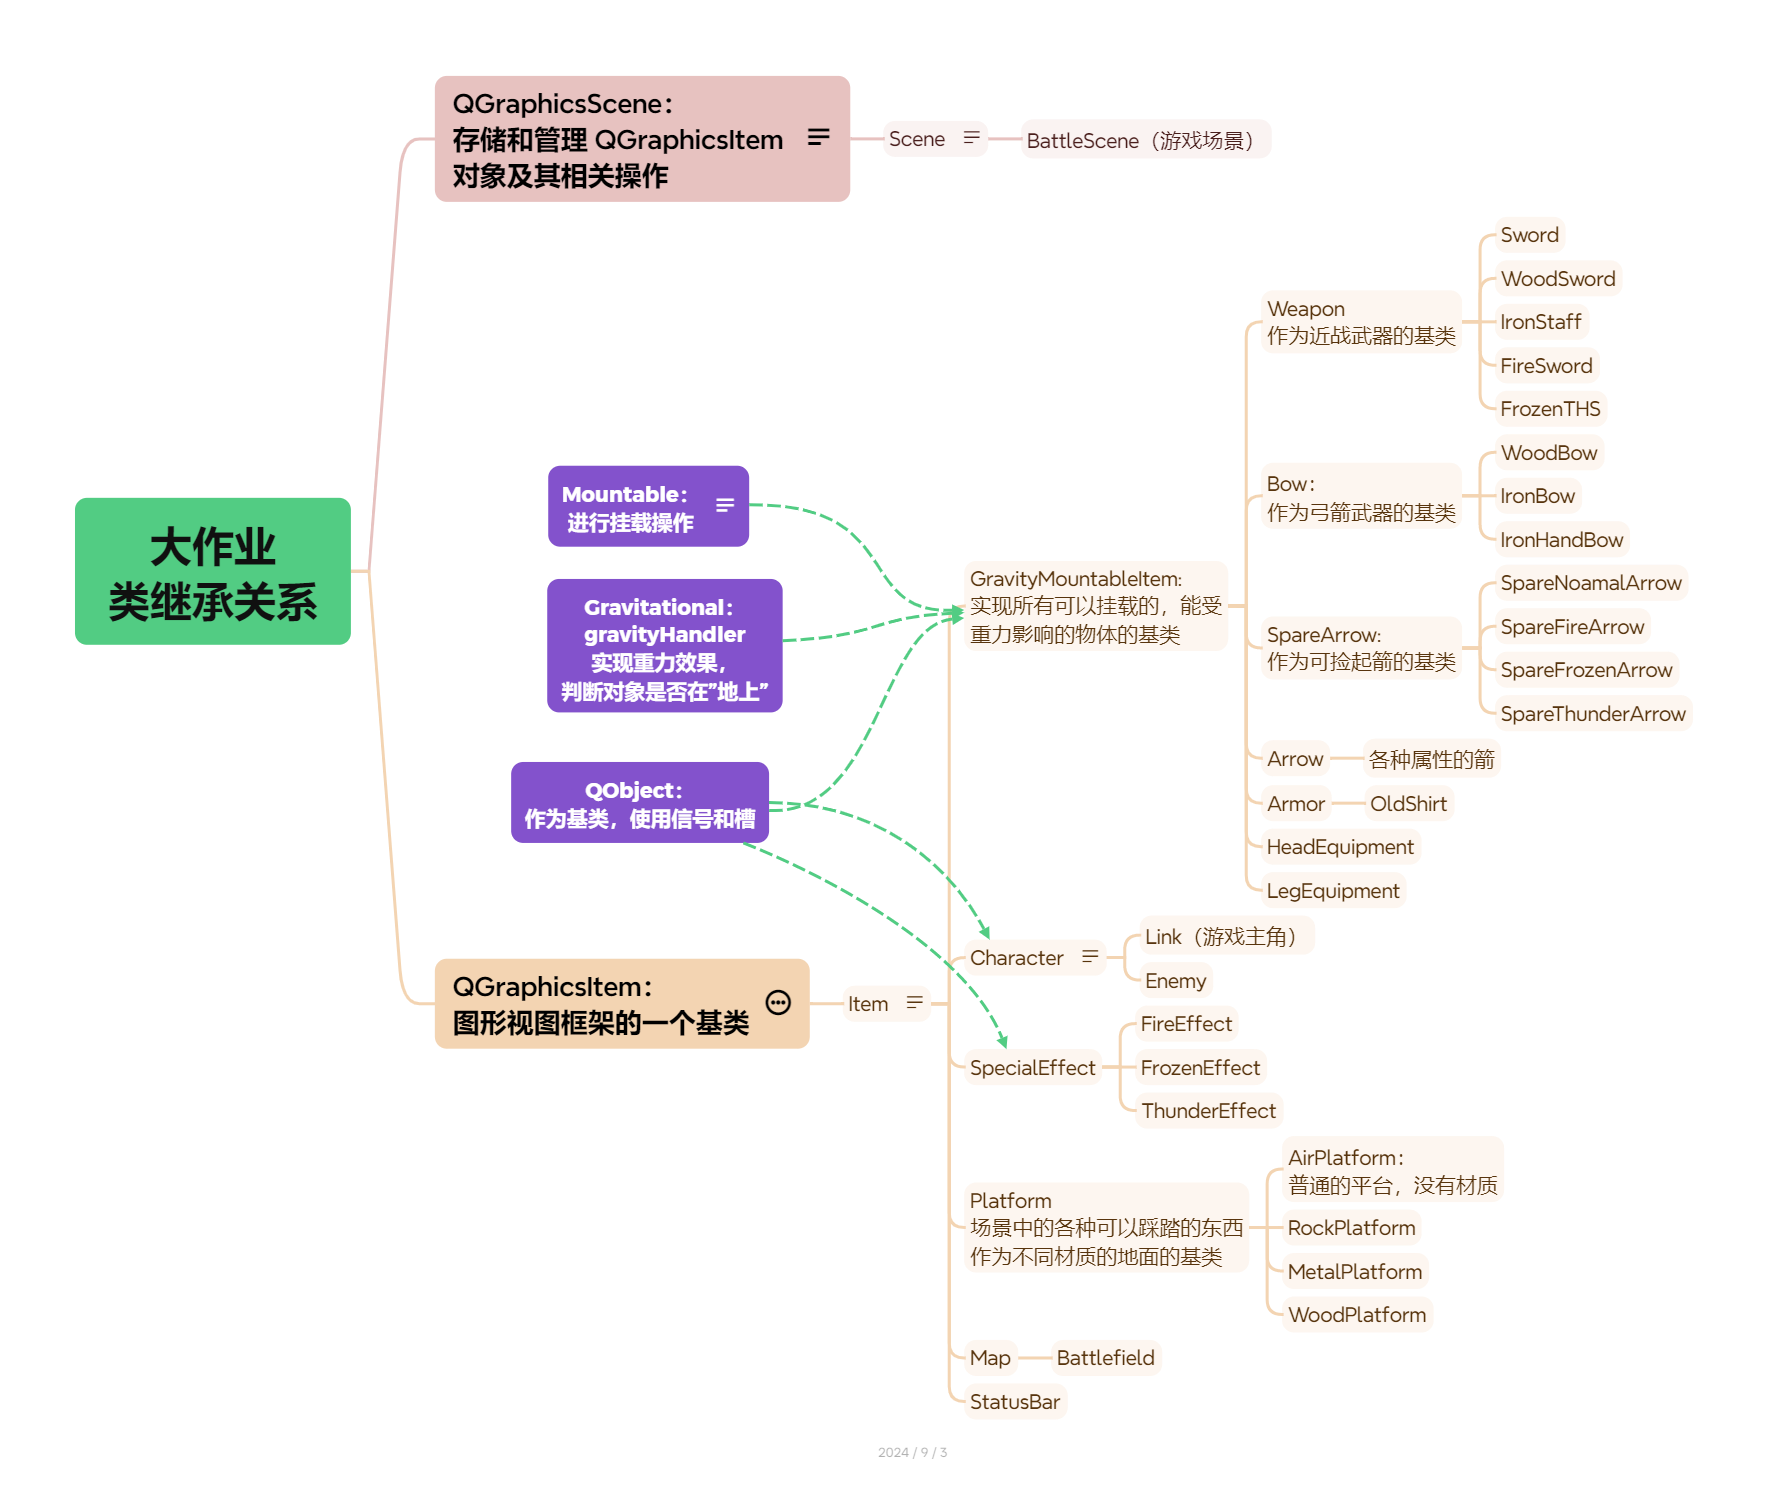
\includegraphics[width=13cm]{image/class_design.png}
    \caption{类设计的思维导图}
    \label{fig:class_design}
\end{figure}

\begin{itemize}
    \item \textbf{QGraphicsScene}:存储和管理 \texttt{QGraphicsItem} 对象及其相关操作,提供了场景中所有图形项的容器。
    \item \textbf{Scene}:管理游戏循环、时间管理、输入处理、对象移动和拾取操作。是具体场景类如 \texttt{BattleScene} 的基类。
    \begin{itemize}
        \item \textbf{BattleScene}:一个具体的游戏场景类,管理战斗场景中的逻辑更新和事件处理。
    \end{itemize}
    \item \textbf{QGraphicsItem}:图形视图框架的一个基类,用于表示所有可以绘制的对象。
    \item \textbf{Item}:继承自 \texttt{QGraphicsItem},定义了游戏中的物体基础行为,如边界、形状和绘制逻辑。
    \begin{itemize}
        \item \textbf{GravityMountableItem}:实现所有可以挂载的、能受重力影响的物体的基类。
        \begin{itemize}
            \item \textbf{Weapon}:近战武器的基类。
            \item \textbf{Bow}:弓箭武器的基类。
            \item \textbf{SpareArrow}:可拾取的箭的基类。
            \item \textbf{Arrow}:各种属性的箭。
            \item \textbf{Armor}:角色护甲的基类。
            \item \textbf{HeadEquipment} 和 \textbf{LegEquipment}:角色头部和腿部装备。
        \end{itemize}
        \item \textbf{Character}:定义角色的基本行为,包括移动、拾取物品、管理装备等。
        \begin{itemize}
            \item \textbf{Link}:主角类。
            \item \textbf{Enemy}:敌人类。
        \end{itemize}
        \item \textbf{SpecialEffect}:定义游戏中的特效,如火焰、冰冻和雷电效果。
        \item \textbf{Platform}:定义游戏中的平台,如普通平台、岩石平台、金属平台、木平台等。
        \item \textbf{Map}:定义游戏中的地图和地形,如战场。
        \item \textbf{StatusBar}:显示角色状态的界面组件。
    \end{itemize}
    \item \textbf{Mountable}:管理对象的挂载状态和逻辑操作。
    \item \textbf{Gravitational}:实现重力效果,判断对象是否在地面上。
\end{itemize}

\section{完成的要求}
\begin{itemize}
    \item 实现了主角的基本控制,包括左右移动(按键1和2)和跳跃(按键3),并支持重力加速度和不同高度的平台。
    \begin{figure}[H]
        \centering
        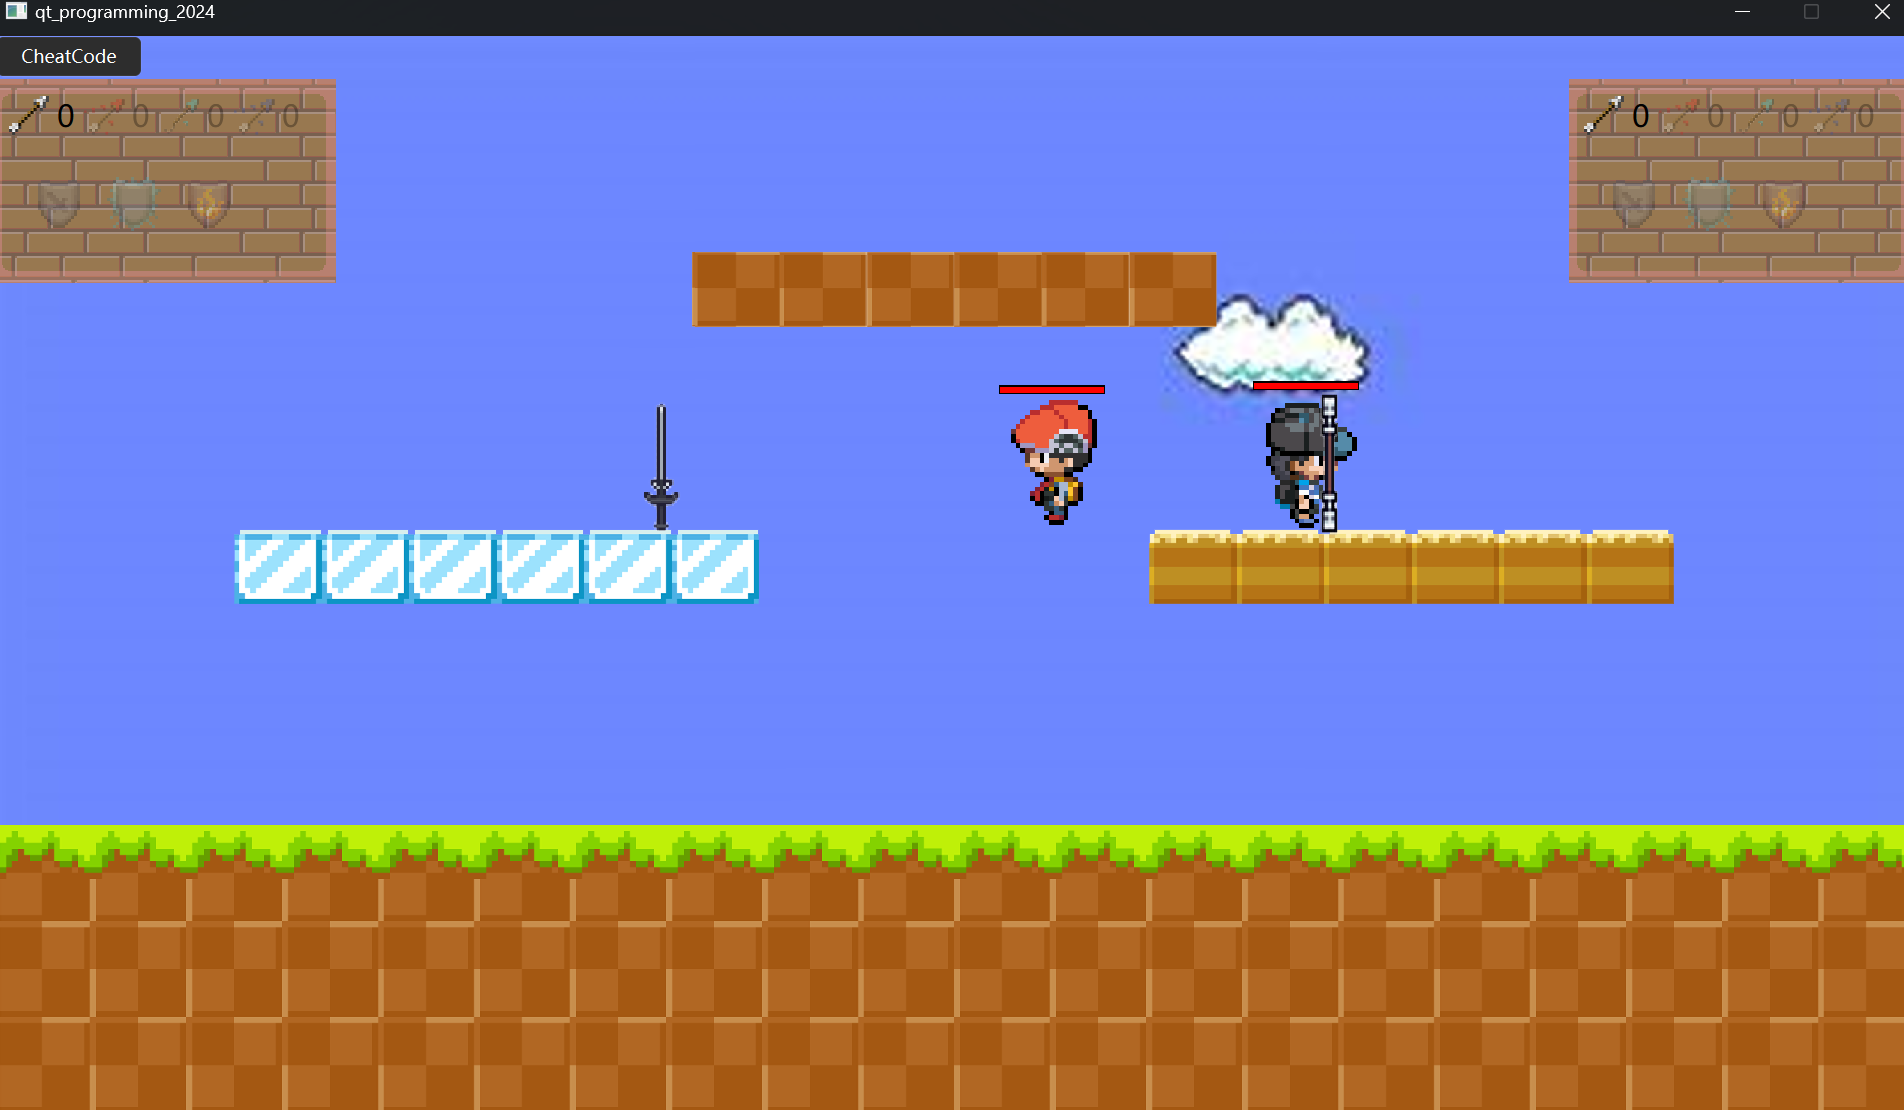
\includegraphics[width=10cm]{image/screenshot_1.png}
        \caption{人物的移动和跳跃实现}
        \label{fig:screenshot_1}
    \end{figure}    
    \item 支持两个玩家同屏对战,各自拥有生命值,生命值为零时游戏结束。
    \begin{figure}[H]
        \centering
        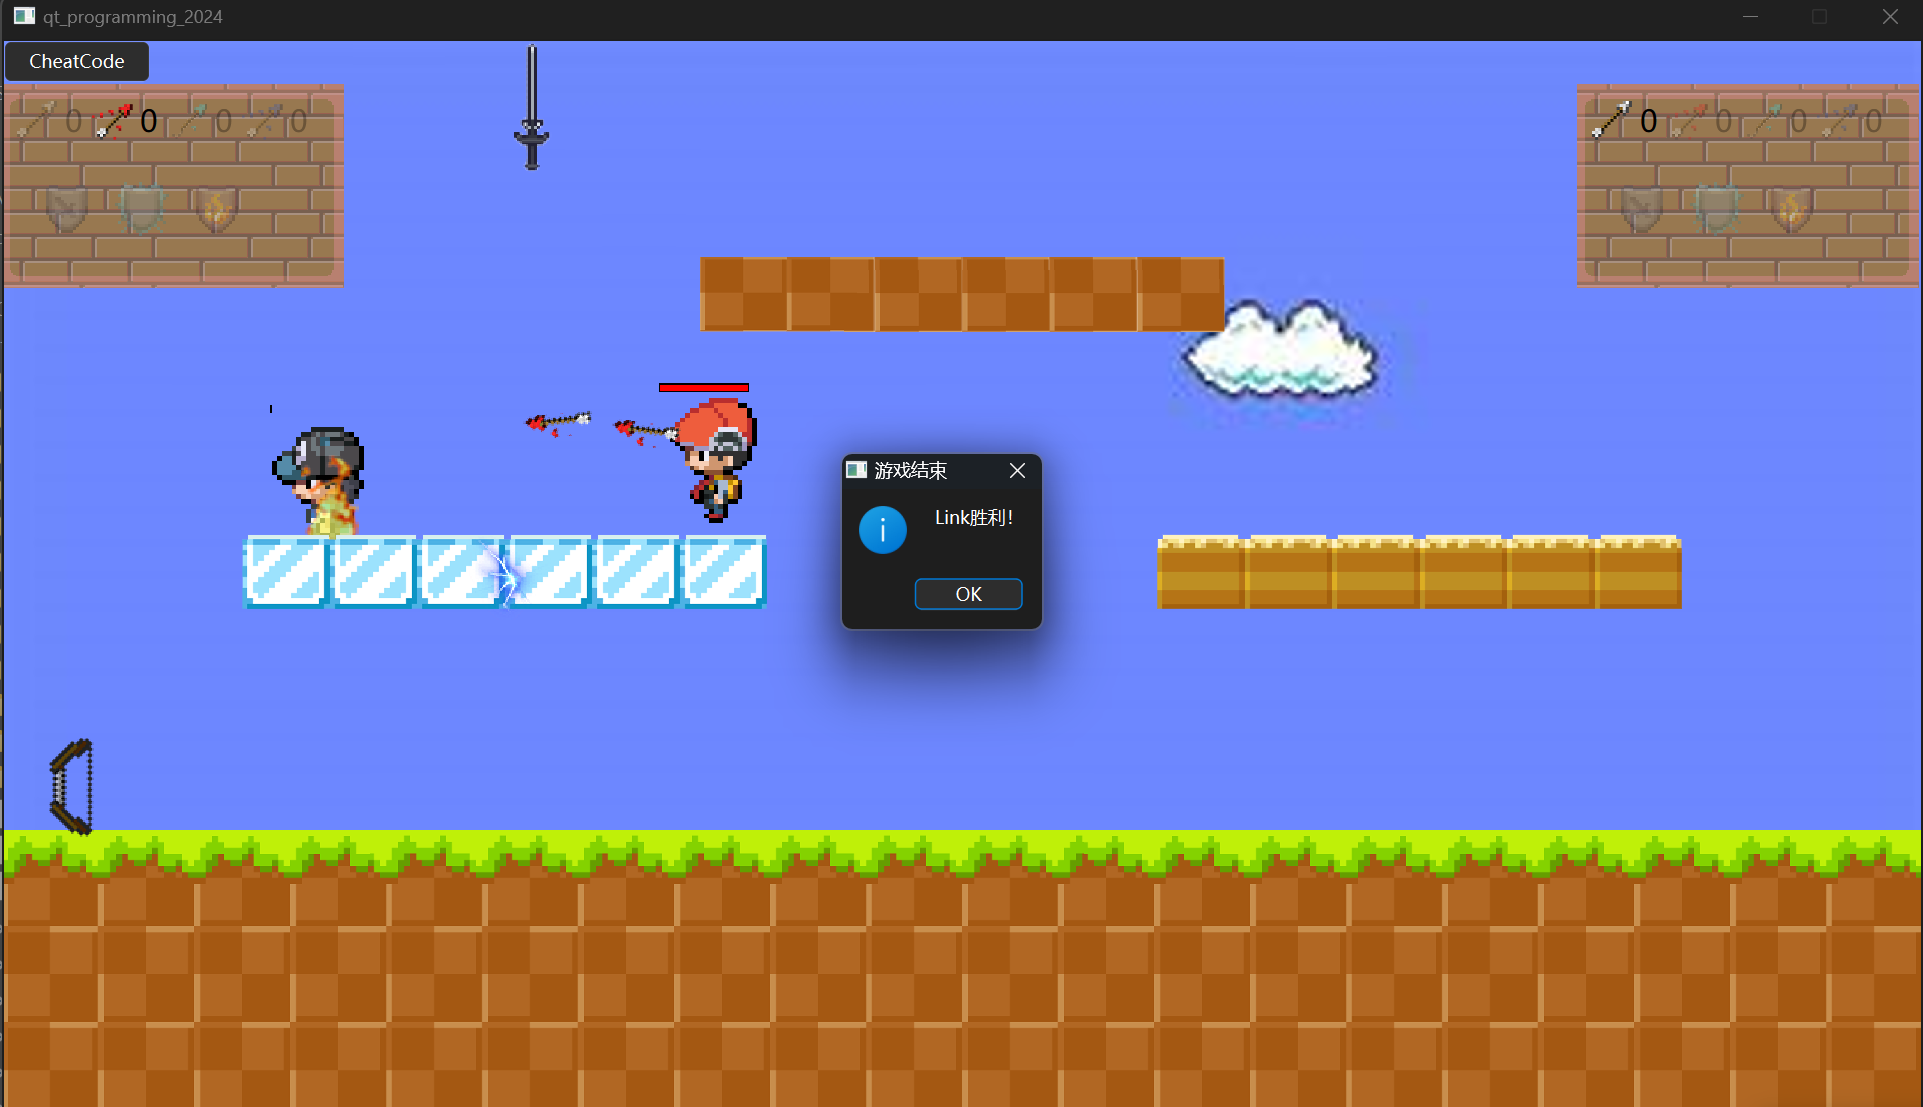
\includegraphics[width=10cm]{image/screenshot_2.png}
        \caption{人物生命值为零时结束游戏}
        \label{fig:screenshot_2}
    \end{figure}
    \item 实现了随机掉落的武器和物品,按键4捡起物品,并具备简单的攻击动画。支持投掷近战武器和在近战武器与弓之间切换。
    \begin{figure}[H]
        \centering
        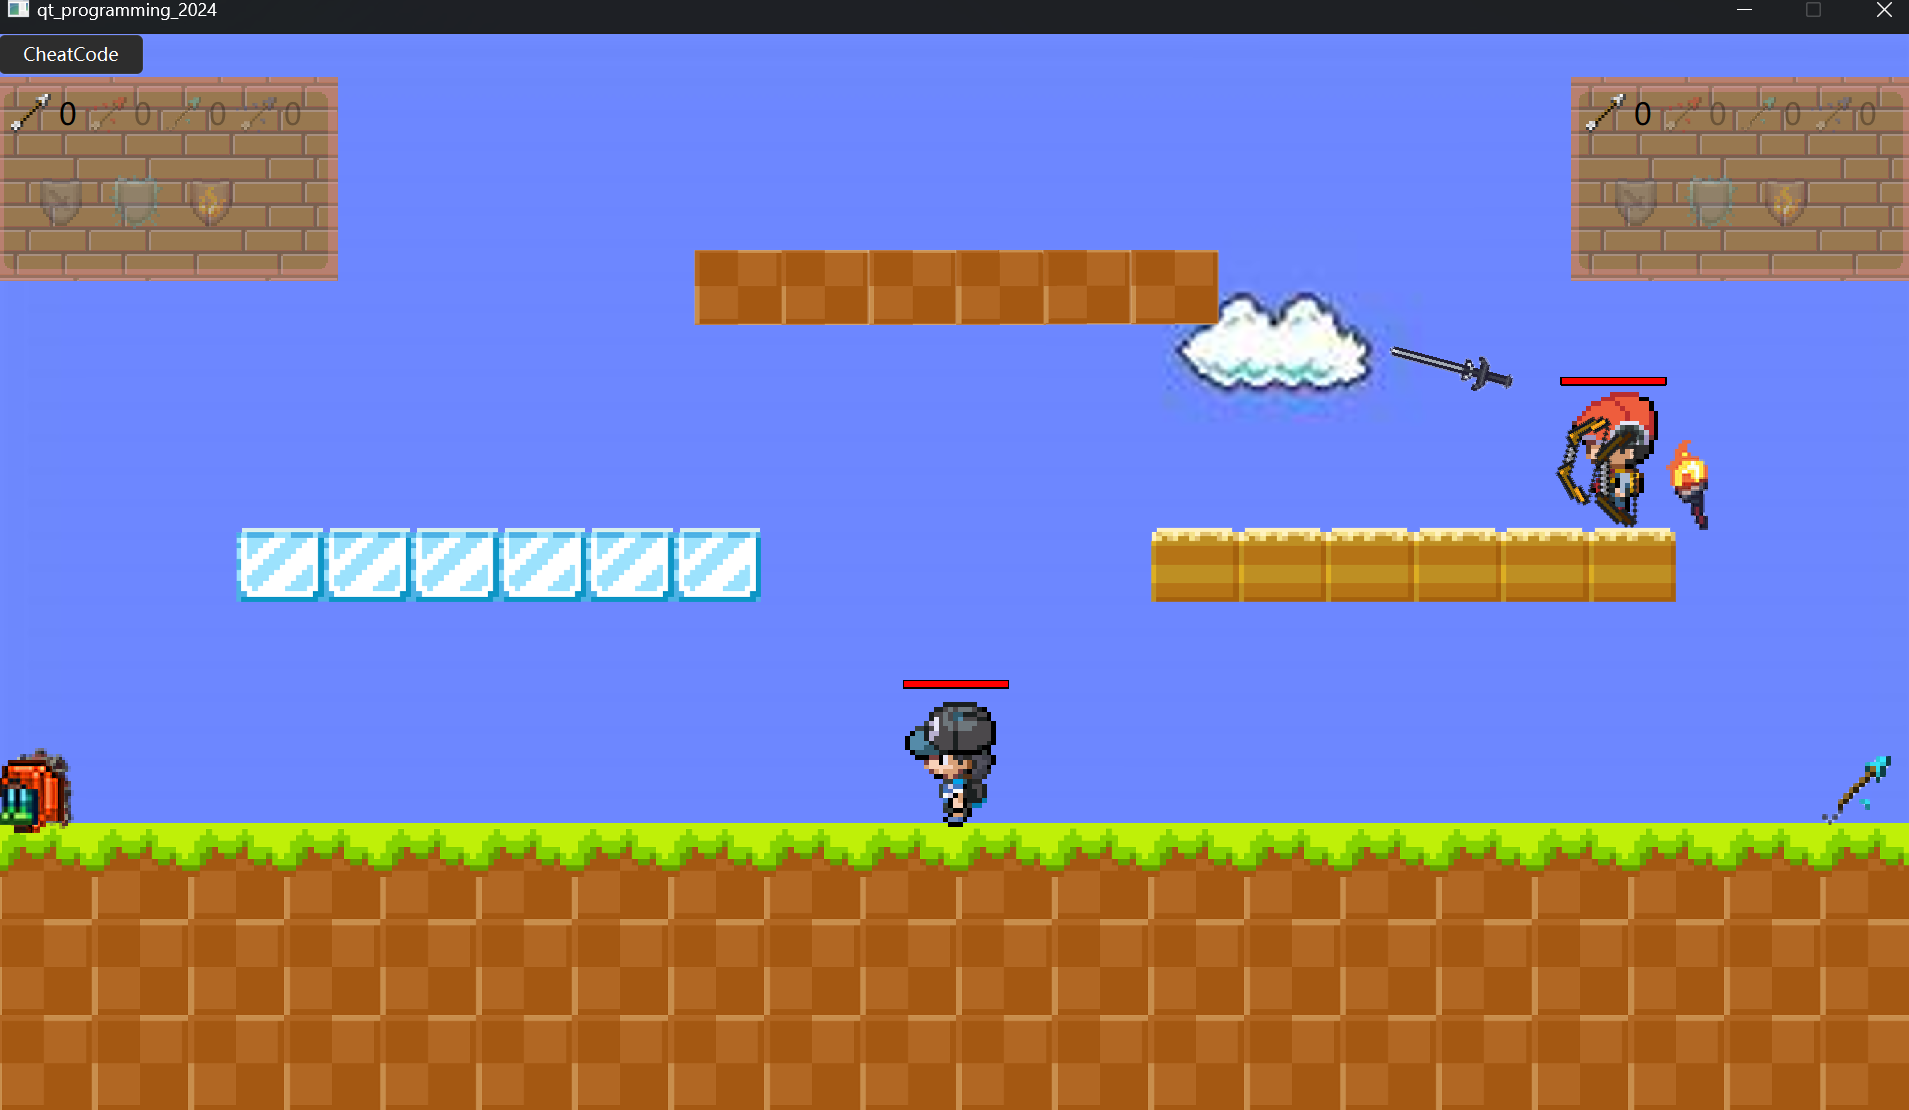
\includegraphics[width=10cm]{image/screenshot_3.png}
        \caption{人物能投掷近战武器并切换武器}
        \label{fig:screenshot_3}
    \end{figure}
    \item 支持不同类型的弓和箭,能够渲染飞行中的箭,并处理箭的射击和弹容量管理。
    \begin{figure}[H]
        \centering
        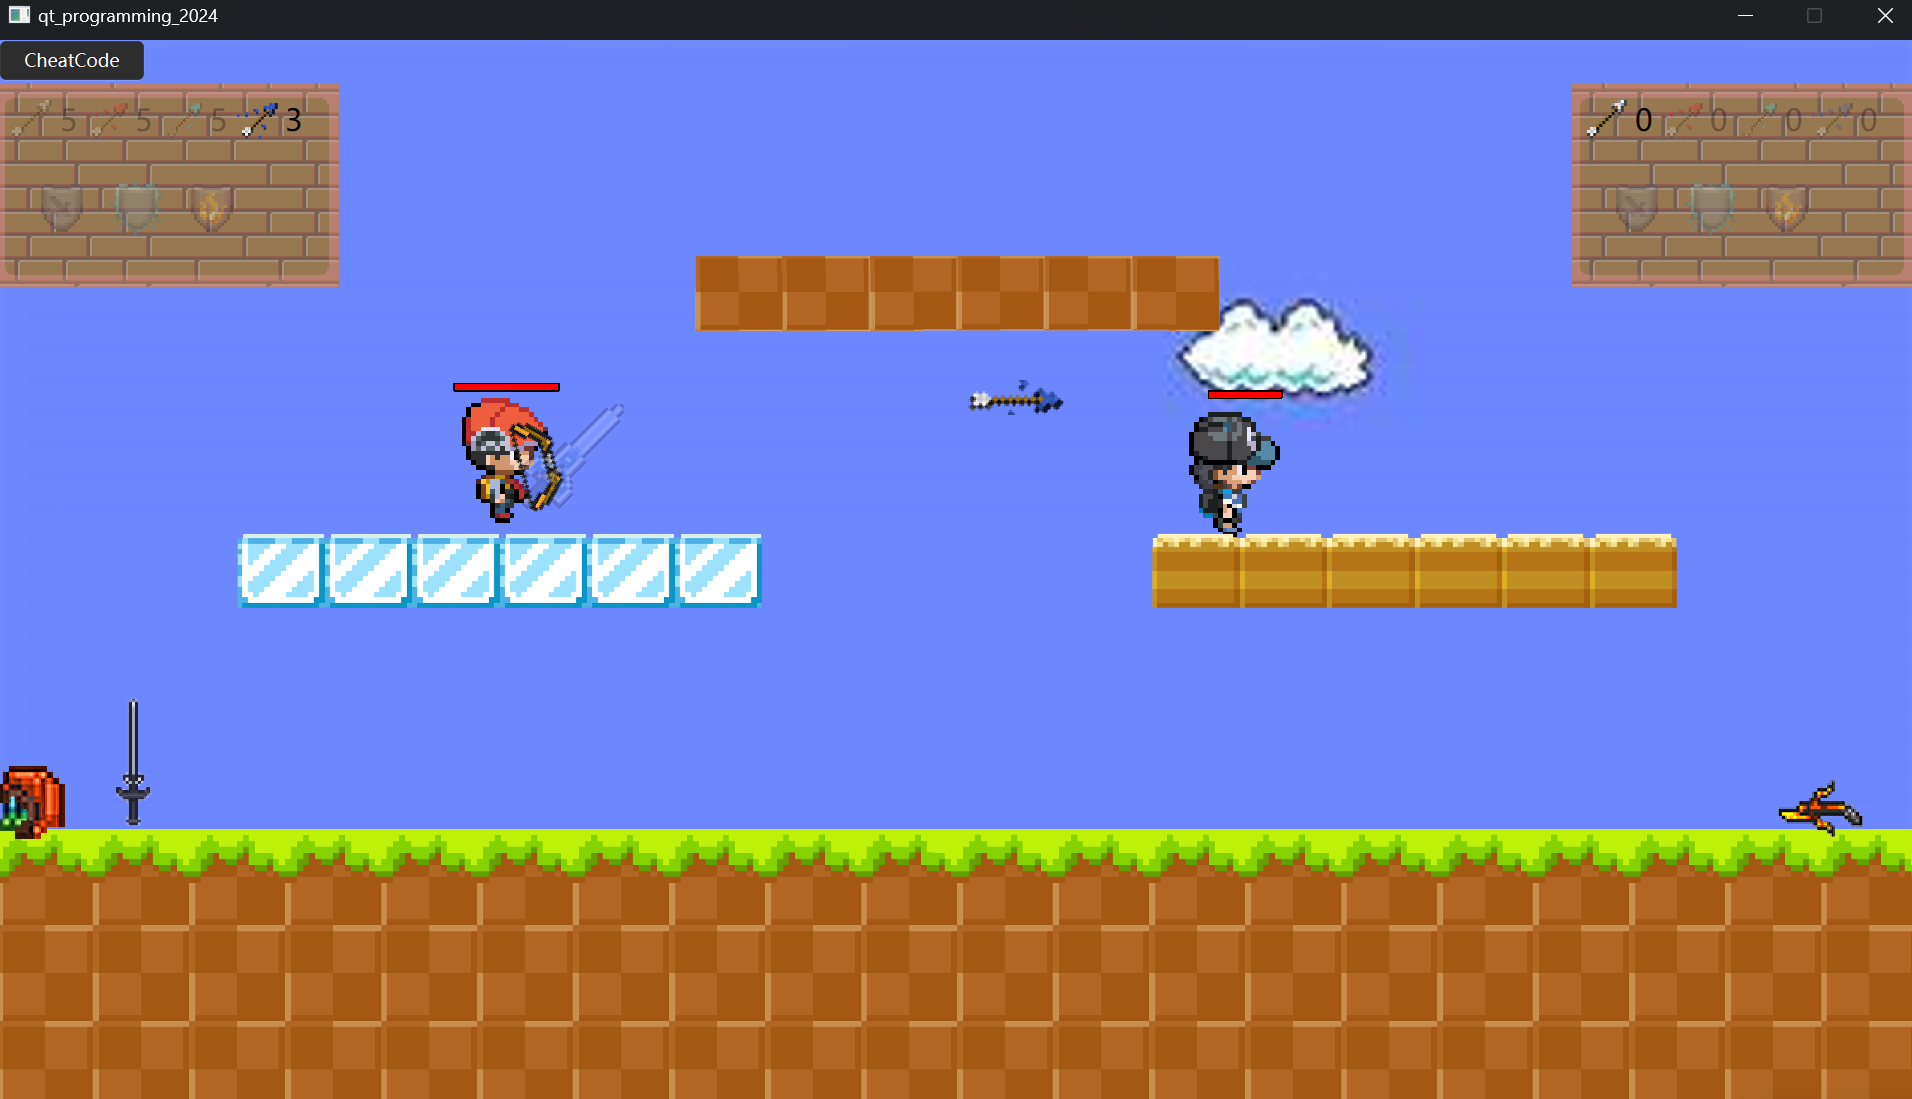
\includegraphics[width=10cm]{image/screenshot_4.png}
        \caption{空中的箭和弹容量管理}
        \label{fig:screenshot_4}
    \end{figure}
    \item 增加了火、冰、电属性的武器及其效果,包括火焰、冰冻和电击状态。
    \begin{figure}[H]
        \centering
        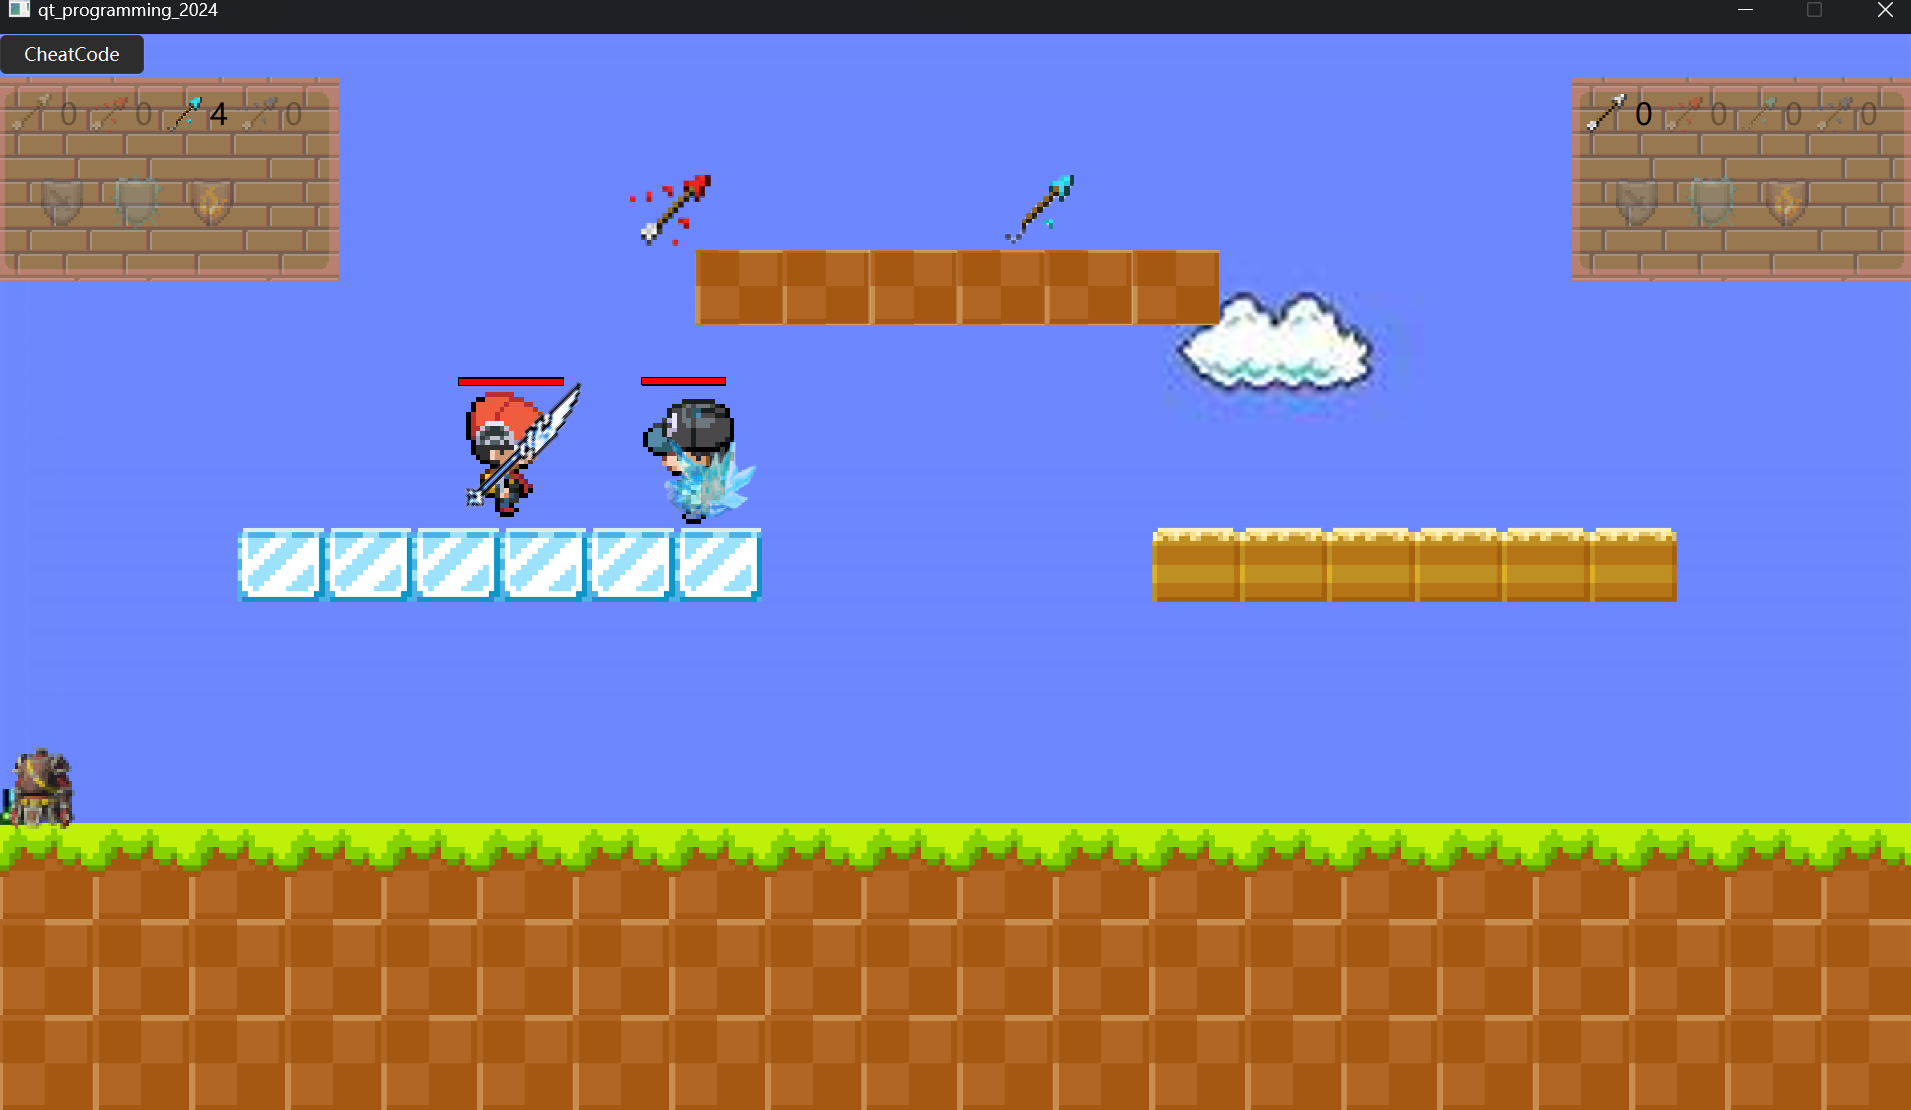
\includegraphics[width=10cm]{image/screenshot_5.png}
        \caption{实现多种元素,图中为冰元素}
        \label{fig:screenshot_5}
    \end{figure}
    \item 实现了盔甲系统,允许玩家捡起并更换盔甲,盔甲提供对火、冰、电的免疫效果。
    \begin{figure}[H]
        \centering
        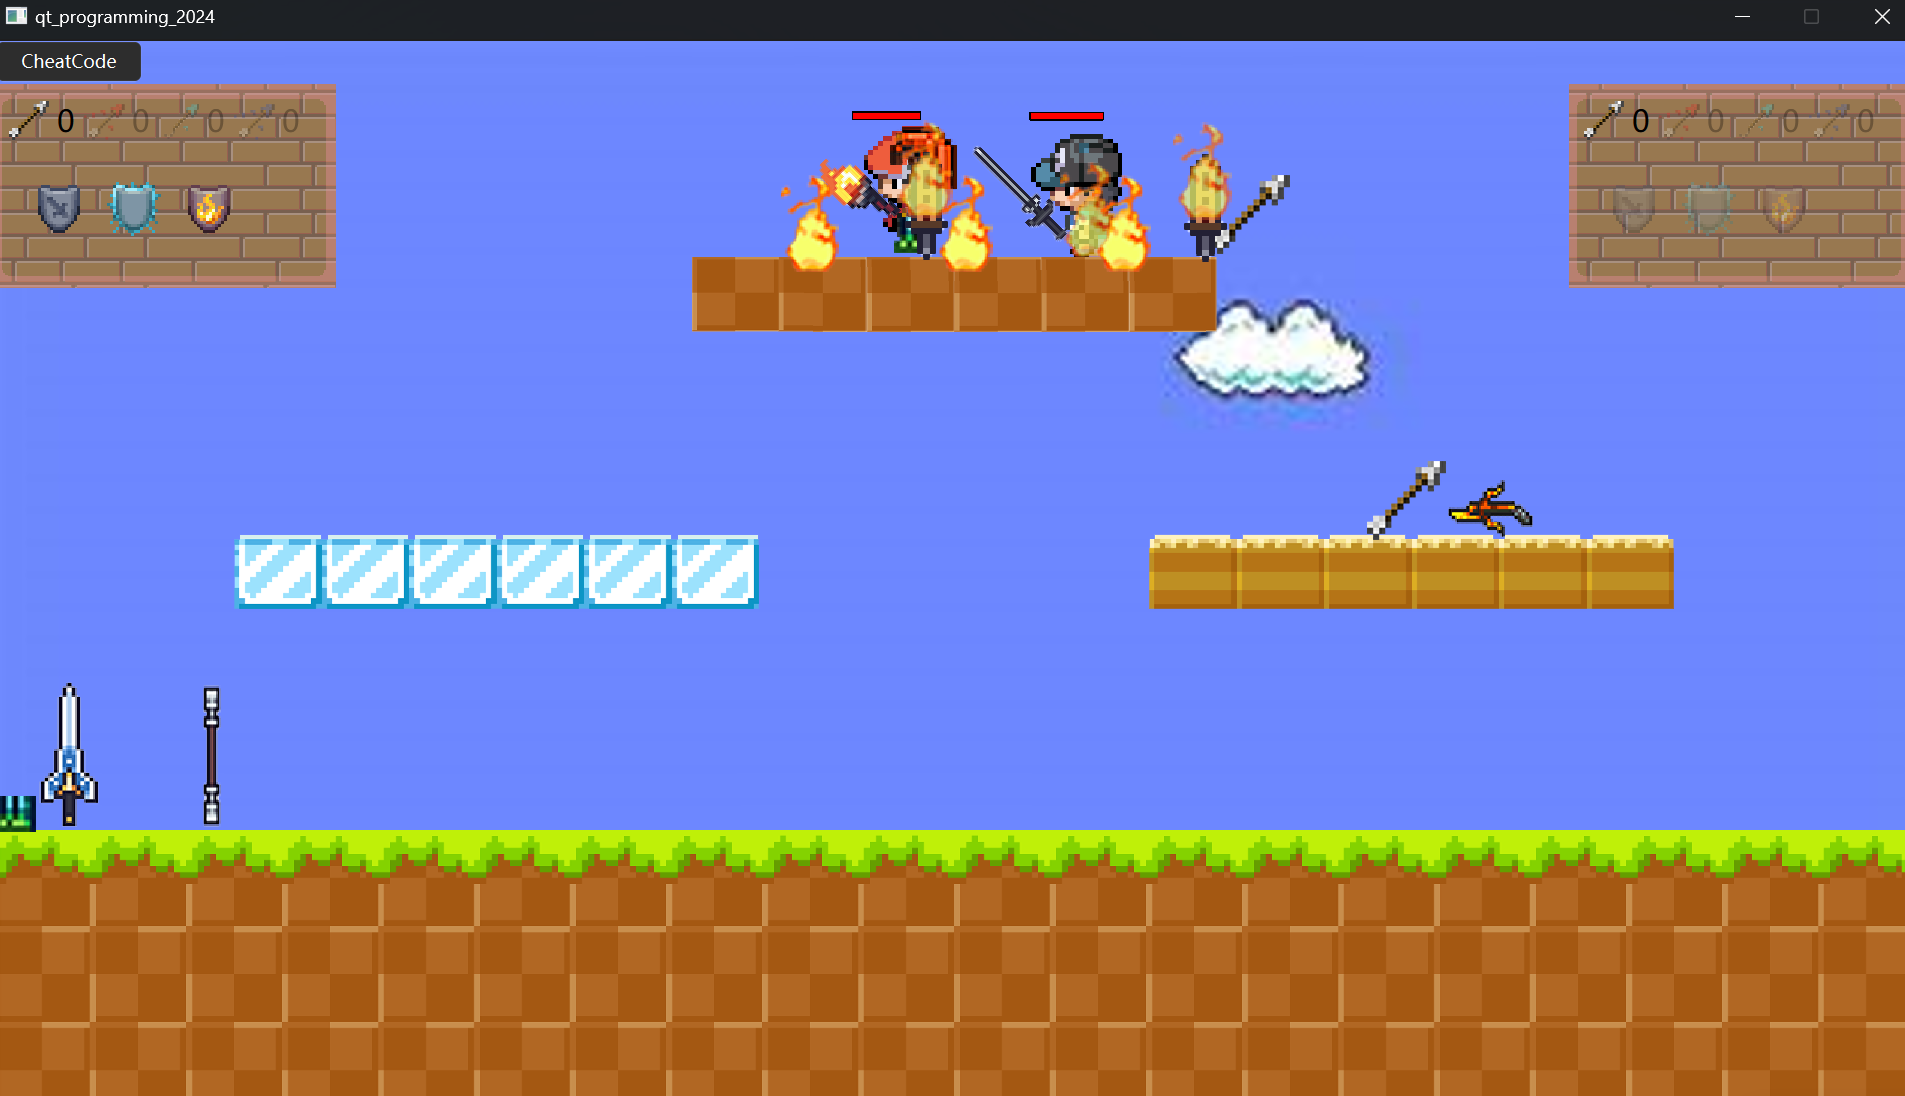
\includegraphics[width=10cm]{image/screenshot_6.png}
        \caption{实现了多种盔甲实现元素防护}
        \label{fig:screenshot_6}
    \end{figure}
\end{itemize}

\section{参考文献}

在本项目中,我们使用了以下库和工具:

\begin{itemize}
    \item \textbf{Qt库}:
    \begin{itemize}
        \item \texttt{QRandomGenerator}: 生成随机数。
        \item \texttt{QDateTime}: 处理日期和时间。
        \item \texttt{QGraphicsItem}: 处理图形项目。
        \item \texttt{QTimer}: 处理定时器。
        \item \texttt{QKeyEvent}: 处理键盘事件。
        \item \texttt{QGraphicsView}: 显示图形视图。
        \item \texttt{QMainWindow}: 主窗口组件。
        \item \texttt{QDialog}: 对话框组件。
        \item \texttt{QLineEdit}: 单行文本编辑器。
        \item \texttt{QPushButton}: 按钮组件。
    \end{itemize}
\end{itemize}

所有这些库的详细信息和使用说明可以在 Qt 官方文档中找到\cite{qt_documentation}。

\begin{thebibliography}{99}
    \bibitem{qt_documentation} Qt Documentation, \textit{Qt 6 Documentation}, available at \url{https://doc.qt.io/qt-6/index.html}.
    \bibitem{qt_examples} Qt Examples and Tutorials, available at \url{https://doc.qt.io/qt-6/qtwidgets-widgets-tutorial.html}.
    \bibitem{qt_wiki} Qt Wiki, available at \url{https://wiki.qt.io/}.
\end{thebibliography}



\end{document}
